%%%%%%%%%%%%%%%%%%%%%%%%%%%%%%%%%%%%%%%%%%%%%%%%%%%%%%%%%%%%%%%%%%%%%%%%%
%
% File: TrickHLASpec.tex
%
% Purpose: TrickHLA Product Specification
%
%%%%%%%%%%%%%%%%%%%%%%%%%%%%%%%%%%%%%%%%%%%%%%%%%%%%%%%%%%%%%%%%%%%%%%%%%

\newcommand\documentHistory{
{\bf Author} & {\bf Date} & {\bf Description} \\ \hline \hline
Edwin Z. Crues & June 2020 & TrickHLA Version 3 \\ \hline
}


% This documentation file's change history includes:
% "REVISED BY name(s)" & "revision DATE" & "revision DESCRIPTION"
%  ------------------     -------------     --------------------

\newcommand\DocumentChangeHistory{
{\bf Revised by} & {\bf Date} & {\bf Description} \\ \hline \hline
}

\documentclass[twoside,11pt,titlepage]{report}

%
% Bring in the amsmath environment
%
\usepackage{amsmath}

%
% Bring in the common page setup
%
\usepackage{trickhlaenv}

%
% Bring in the common math nomenclature
%
\usepackage{trickhlamath}

%
% Bring in the model-specific commands with requirement labels
%
\usepackage[Reqt]{TrickHLA}

%
% Bring in the graphics environment
%
\usepackage{graphicx}

%
% Bring in listing environment
%
\usepackage{paralist}

%
% Bring in the hyper ref environment
%
\usepackage[colorlinks]{hyperref}
%  keywords for pdfkeywords are separated by commas
\hypersetup{
   pdftitle={\TrickHLA\ Product Specification},
   pdfauthor={Edwin Z. Crues \\ and \\ Daniel E. Dexter},
   pdfkeywords={\TrickHLA, Product Specification},
   pdfsubject={\TrickHLA\ Product Specification}}

\begin{document}

%%%%%%%%%%%%%%%%%%%%%%%%%%%%%%%%%%%
% Front matter
%%%%%%%%%%%%%%%%%%%%%%%%%%%%%%%%%%%
\pagenumbering{roman}

\docid{DD.mm.20}
\docrev{1.0}
\date{June 2020}
\modelname{\TrickHLA}
\doctype{Product Specification}
\author{Edwin Z. Crues \\ and \\ Daniel E. Dexter}
\managers{
  Edwin Z. Crues \\ Project Manager \\
  Michael T. Red \\ Simulation and Graphics Branch Chief (ER7) \\
  Robert O. Ambrose \\ Software, Robotics, and Simulation Division Chief}
\pdfbookmark{Title Page}{titlepage}
\makeTrickhlaenvTitlepage

%%%%%%%%%%%%%%%%%%%%%%%%%%%%%%%%%%%%%%%%%%%%%%%%%%%%%%%%%%%%%%%%%%%%%%%%%
%
% Purpose: Abstract for TrickHLASpec
%
% Author: David A. Hasan - 22 April 2007
%
% Modified:
%
%
%%%%%%%%%%%%%%%%%%%%%%%%%%%%%%%%%%%%%%%%%%%%%%%%%%%%%%%%%%%%%%%%%%%%%%%%%

\pdfbookmark{Abstract}{abstract}
\begin{abstract}
The \TrickHLA\ model provides a simplified interface to the
IEEE-1516 High Level Architecture (HLA) \cite{IEEE1516:API}
for use in the Trick Simulation Environment.
It allows developers to concentrate on simulation development
without needing to be an HLA expert.
The model is heavily data driven
and based on a simple API C++ making it relatively easy to take an existing
Trick simulation and make it HLA aware.
This document provides a high-level overview of the model.
\end{abstract}


\pdfbookmark{Contents}{contents}
\tableofcontents
\vfill

\pagebreak

%%%%%%%%%%%%%%%%%%%%%%%%%%%%%%%%%%%
% Main Document Body
%%%%%%%%%%%%%%%%%%%%%%%%%%%%%%%%%%%
\pagenumbering{arabic}

%%%%%%%%%%%%%%%%%%%%%%%%%%%%%%%%%%%%%%%%%%%%%%%%%%%%%%%%%%%%%%%%%%%%%%%%%
%
% File: TrickHLASpec-Intro.tex
%
% Purpose: TrickHLA Product Specification - Intro Chapter
%
%%%%%%%%%%%%%%%%%%%%%%%%%%%%%%%%%%%%%%%%%%%%%%%%%%%%%%%%%%%%%%%%%%%%%%%%%

%----------------------------------
\chapter{Introduction}\label{sec:intro}
%----------------------------------

%%%%%%%%%%%%%%%%%%%%%%%%%%%%%%%%%%%%%%%%%%%%%%%%%%%%%%%%%%%%%%%%%%%%%%%%%
%
% Purpose: Introduction for TrickHLA
%
% Author: Edwin Z. Crues - 19 May 2020
%
% Modified:
%
%
%%%%%%%%%%%%%%%%%%%%%%%%%%%%%%%%%%%%%%%%%%%%%%%%%%%%%%%%%%%%%%%%%%%%%%%%%

The objective of \TrickHLA\ is to simplify the process of providing simulations
built with the Trick Simulation Environment\cite{Trick:Documentation} with
the ability to participate in distributed executions using the High Level
Architecture (HLA)\cite{IEEE1516:FRAMEWORK}. This allows a simulation developer
to concentrate on the simulation and not have to be an HLA expert.
\TrickHLA\ is data driven and provides a simple API making it relatively easy
to take an existing Trick simulation and make it HLA capable.


\section{Identification of Document}
This document describes the design of the \TrickHLA\ developed
for use in the Trick Simulation Environment.
This document adheres to the documentation standards
defined in NASA Software Engineering Requirements Standard \cite{NASA:SWE}.

\section{Scope of Document}
This document provides information on the algorithms used in and
the design of the source code associated with \TrickHLA.
This includes references to relevant Trick and HLA documents.

\section{Purpose and Objectives of Document}
The purpose of this document is to provide a thorough understanding of the
\TrickHLA\ product and its underlying architecture and design.

\section{Documentation Status and Schedule}
The information in this document is current with the \TrickHLAid\
implementation of \TrickHLA. 
Updates will be kept current with module changes.

\begin{tabular}{||l|l|l|} \hline
\documentHistory
\end{tabular}

\begin{tabular}{||l|l|l|} \hline
\DocumentChangeHistory
\end{tabular}

\section{Document Organization}
This document is organized into the following sections:

\begin{description}

\item[Chapter \ref{sec:intro}: Introduction] -
Identifies this document, defines the scope and purpose, present status,
and provides a description of each major section.

\item[Chapter \ref{sec:docs}: Related Documentation] -
Lists the related documentation that is applicable to this project.

\item[Chapter \ref{sec:architectural_design}: Architectural Design] -
Presents the top-level concepts behind \TrickHLA.

\item[Chapter \ref{sec:math_formulations}: Mathematical Formulations] -
Presents the mathematical formulations implemented by \TrickHLA.

\item[Chapter \ref{sec:interface_design}: Interface Design] -
Describes the main interfaces to the \TrickHLA\ model.

\item[Chapter \ref{sec:functional_design}: Functional Design] -
Presents the detailed design of the model.

\item[Chapter \ref{sec:versions}: Version Description] -
Identifies the configuration-managed items that comprise \TrickHLA.

\item[Bibliography] -
Informational references associated with this document.

\end{description}


%%%%%%%%%%%%%%%%%%%%%%%%%%%%%%%%%%%%%%%%%%%%%%%%%%%%%%%%%%%%%%%%%%%%%%%%%
%
% File: TrickHLASpec-RelatedDocs.tex
%
% Purpose: TrickHLA Product Specification - Related Documentation chapter
%
%%%%%%%%%%%%%%%%%%%%%%%%%%%%%%%%%%%%%%%%%%%%%%%%%%%%%%%%%%%%%%%%%%%%%%%%%

\chapter{Related Documentation}\label{sec:docs}

\section{Parent Documents}
The following documents are parent to this document:

\begin{itemize}
\item{\href{file:\TRICKHLAHOME/docs/TrickHLA.pdf}
           {\em Trick High Level Architecture (\TrickHLA)}}
\cite{trickhlaenv:TrickHLA}
\end{itemize}

\section{Applicable Documents}
The following documents are referenced herein and are directly
applicable to this document:

\begin{itemize}
\item{\href{file:TrickHLAReqt.pdf}
           {\em \TrickHLA\ Product Requirements}}
\cite{trickhlaenv:TrickHLAReqt}

\item{\href{file:TrickHLAUser.pdf}
           {\em \TrickHLA\ User Guide}}
\cite{trickhlaenv:TrickHLAUser}

\item{\href{file:TrickHLAIVV.pdf}
           {\em \TrickHLA\ Inspection, Verification, and Validation}}
\cite{trickhlaenv:TrickHLAIVV}

\item{\em Trick Simulation Environment: Installation Guide}
\cite{Trick:Install}

\item{\em Trick Simulation Environment: Tutorial}
\cite{Trick:Tutorial}

\item{\em Trick Simulation Environment: Documentation}
\cite{Trick:Documentation}

\item{\em NASA Software Engineering Requirements}
\cite{NASA:SWE}
\end{itemize}

\section{Information Documents}
The following documents provide supporting material for understanding the
concepts in this document:

\begin{itemize}
\item{\em Asynchronous distributed simulation via a sequence of parallel computations} 
\cite{art:chandy-misra}
\item{\em Parallel Discrete Event Simulation} 
\cite{art:fujimoto-acm}
\end{itemize}

%%%%%%%%%%%%%%%%%%%%%%%%%%%%%%%%%%%%%%%%%%%%%%%%%%%%%%%%%%%%%%%%%%%%%%%%%
%
% File: TrickHLASpec-ArchDesign.tex
%
% Purpose: TrickHLA Product Specification - Architectural Design chapter
%
%%%%%%%%%%%%%%%%%%%%%%%%%%%%%%%%%%%%%%%%%%%%%%%%%%%%%%%%%%%%%%%%%%%%%%%%%

\chapter{Architectural Design}\label{sec:architectural_design}

This chapter presents the high-level concepts behind \TrickHLA\ and
summarizes the model's architecture.

\section{Summary}

The \TrickHLA\ model provides developers a
relatively simple means of integrating HLA into Trick simulations.
The model code is written in C++, since the HLA APIs are in C++.
The architecture reflects this C++ foundation.
In addition, since the model is intended for use with Trick,
the architecture is also based on Trick-specific concepts, namely a
Trick {\ttfamily sim\_object} and default data input files.

\section{Background}

\subsection{Purpose and Scope}
\paragraph{Purpose.}
The \TrickHLA\ model presents a high-level means by which simulation
developers may integrate HLA into a simulation, thereby incorporating
it into a distributed federation of simulations.
In particular, the model makes this integration easier than would
otherwise be the case, since the HLA programming interface is fairly
complex and difficult to master.

\paragraph{Scope.}
The \TrickHLA\ model is intended for use only in Trick-based simulations.
It consists of
\begin{itemize}
  \item{several C++ classes,}
  \item{a Trick {\ttfamily sim\_object}, and}
  \item{a default data file for that {\ttfamily sim\_object}.}
\end{itemize}

\subsection{Goals and Objectives}

\paragraph{Goals.}
The general goal of the \TrickHLA\ model is to enable developers to build 
distributed HLA-based simulations with a minimum of HLA expertise.

\paragraph{Objectives.}
The specific objective of \TrickHLA\ is to provide programming tools
that allow simulation developers to easily integrate HLA into a simulation.

The module includes C++ classes and a {\ttfamily sim\_object} 
which provide a high level interface to HLA --- 
one that is easier to use and understand.
Furthermore, the tight integration of HLA {\em publish} and {\em subscribe}
capabilities with Trick enables developers to automatically send and receive 
HLA data using Trick input files instead of code.
Other HLA capabilities
(e.g., sending and receiving {\em interactions} 
and managing attribute {\em ownership})
are handled by \TrickHLA\ classes and functions which must be invoked
explicitly but are easier to work with than the standard HLA functions.

\subsection{Concepts and Terminology}

This section summarizes some key Trick and HLA terminology and concepts
in order to make the subsequent presentation of the \TrickHLA\ model
easier to understand.

\begin{description}
\item[Trick.]
Trick is a simulation environment used in NASA and developed at
Johnson Space Center.
The architectural model for this software is as defined in, and
required by, the Trick Simulation Environment. 
See references \cite{Trick:Documentation} and \cite{Trick:Tutorial}
for more information on Trick.
Trick-based simulations consist of {\em models} which roughly speaking
are sets of related data and functions which operate on them.
The \TrickHLA\ model is a Trick model in this sense,
and it consists of sets of data and functions which simplify access to HLA.

\item[Data Driven Mechanisms.]
\label{sec:data-driven-mechanisms}
In what follows,
we sometimes refer to data driven mechanisms for accomplishing a task.
By this we mean that the task may be specified in a Trick input file
rather than by writing C or C++ code to handle the task.
One of the useful aspects of Trick is that the simulations it creates are
aggressively data-driven, making it possible to change many simulation 
parameters through input files instead of changing source code and rebuilding
the simulation binary.
The \TrickHLA\ model presents data-driven mechanisms for some (but not all)
HLA tasks.

\item[High Level Architecture (HLA).]
The High Level Architecture (HLA) is an IEEE standard (IEEE-1516)
which defines a set of {\em services} to facilitate the development
of distributed systems.
More information is available in references
\cite{IEEE1516:FRAMEWORK}, \cite{IEEE1516:API}, \cite{IEEE1516:OMT}, and
\cite{IEEE1730:DSEEP}.
The \TrickHLA\ model presents a Trick-friendly interface to the relatively
complex HLA application programming interface (API).

\item[Federates and Federations.]
The distributed system in HLA is refered to as a {\em federation}. 
Each federation has a name, and there may be many federations in existence
at the same time.
Each participant in a particular federation is refered to as a {\em federate}.
A federate may {\em join} one or more federations.
Federates have names, which must be unique in each federation to which they belong.
The \TrickHLA\ model provides a data-driven mechanism for turning a Trick
simulation into an HLA federate and joining the appropriate HLA federation.

\item[Publish and Subscribe.]
The publish/subscribe model of data distribution is one in which
the data in a system are given names which allow {\em publishers} to
set new values for the data and make them available to {\em subscribers}
who must explicitly indicate their interest in specific data (by name)
in order to receive them.
Publish/subscribe systems allow a single publisher to distribute
data to many subscribers without being aware of the specific recipients, 
since subscribers usually register their interest with the underlying 
middleware instead of directly contacting the publisher.
In HLA, the term {\em publish} is used rather unconventionally to indicate
a federate's intent to eventually generate data values. 
The actual act of generating those data values is called {\em reflection}.
The \TrickHLA\ model provides a data-driven mechanism for associating
Trick simulation data with HLA,
allowing simulations to publish/reflect and subscribe data without writing
any code to do so.

\item[Classes, Objects and Attributes.]
In HLA, an {\em object class} is an abstract specification for how some data may
be organized. 
A class consists of various constituents called {\em attributes}.
Instances of a particular HLA object class are called {\em object instances}.
Is is these instances which actually hold data values.
In HLA classes and their instances are meant to be model persistent data,
i.e., things in the simulation domain that exist and have values that continue
to exist over time.
The \TrickHLA\ model provides a data-driven mechanism to associate attributes 
with Trick simulation data.

\item[Interactions and Parameters.]
In HLA, messages can be sent between federates that are not associated with things
that exist over time in the simulation domain.
These are called {\em interactions}.
Like classes, they consist of various constituents, but interaction constituents
are called {\em parameters}.
Interactions and their parameters are used to model transient data.
The \TrickHLA\ model provides a data-driven mechanism to associate parameters 
with Trick simulation data.
The \TrickHLA\ model has functions which may be used to send interactions from
a simulation to other federates in the federation.
It also provides an abstract C++ class which may be subclassed by simulation
developers in order to specify simulation-specific handling of incoming interactions.

\item[Attribute Ownership.]
In HLA, object attributes may be {\em owned} by a particular federate, 
which means that the data values for that attribute are the responsibility
of that federate.
Only one federate may own an attribute at a time; however, the ownership of an
attribute may be transferred from federate to federate during the execution of
the federation.
This transfer of ownership is refered to as {\em ownership management}.
The \TrickHLA\ model has functions which may be used to initiate an ownership
transfer.
(A current attribute owner may {\em push} ownership away,
and a non-owner may {\em pull} ownership from the current owner.)
The model also provides an abstract C++ class which may be subclassed by simulation
developers in order to specify simulation-specific handling of ownership transfers.

\item[Federation Object Model (FOM).]
Each federation must have a single FOM which specifies the object classes, 
attributes, interactions, and parameters which are exchanged during the
federation's execution.
This information is captured in an XML file refered to as the {\em FOM file}.
The \TrickHLA\ model provides a data-driven mechanism to associate a particular
FOM file with a simulation.

\item[Time Management and Lookahead.]
One of the challenges of distributed computing is how one goes about defining
a consistent value of time. 
One of the major aspects of HLA is its {\em time management} services which
allow distributed simulations to proceed concurrently yet have a consistent notion
of time. 
The time management services are typically implemented on top of the
Chandy-Misra-Bryant protocol\cite{art:chandy-misra}
The performance of this protocol is affected significantly by a 
{\em time lookahead} parameter\cite{art:fujimoto-acm}
which is a time interval {\em into the future} to which a federate can predict
(or extrapolate) its current state.
The use of lookahead is a fundamental aspect of HLA simulations.
It is how simulations can reliably proceed in parallel without deadlocking.
The \TrickHLA\ model provides a data-driven mechanism for specifying the lookahead
to be associated with the simulation.

\end{description}

\section{Architectural Overview}

This section provides a very high-level view of the \TrickHLA\ model.
Finer details of this model are presented in
Chapters \ref{sec:interface_design} and \ref{sec:functional_design}.
The model can be described as three layers
as depicted in Figure~\ref{fig:TrickHLA-layers}
%
\begin{figure}[h]
  \begin{center}
    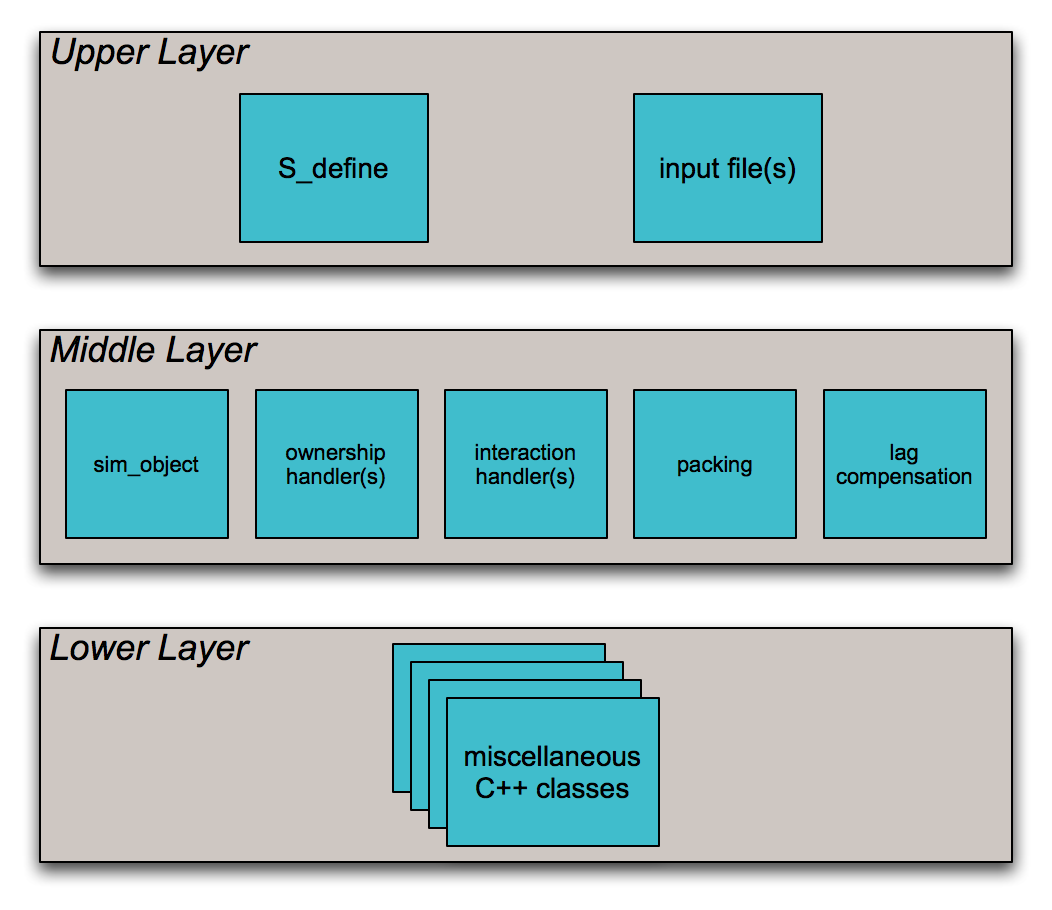
\includegraphics[width=4.5in]{TrickHLA-layers.png}
  \end{center}
\caption{\TrickHLA\ Layers}
\label{fig:TrickHLA-layers}
\end{figure}
%

\subsection{The Upper Layer}

The upper layer of the \TrickHLA\ model consists of simulation-specific
artifacts\footnote{
In a sense, these are not elements of the model, since they are not artifacts delivered 
as part of the model, but since they are important in understanding how the model works, 
we have chosen to explicitly include them in this discussion.}
which must be modified in order to use the model.
These are discussed in the following sections.

\subsubsection{The {\ttfamily S\_define} File}

To integrate \TrickHLA\ into a Trick simulation, the simulation's {\ttfamily S\_define} file
must be modified to include HLA-specific data structures and jobs.
To a large extent, this can be accomplished by inserting the default
\TrickHLA\ {\ttfamily sim\_object} (see below) into the {\ttfamily S\_define} file.
However,
in order to use HLA interactions or ownership management, 
additional {\em handler} data structures (see below) must be inserted into the 
{\ttfamily S\_define} in addition to the {\ttfamily sim\_object}.

\subsubsection{The Input Files}

As discussed on page~\pageref{sec:data-driven-mechanisms},
Trick is a data-driven system. 
Accordingly, most parameters related to the \TrickHLA\ model are initialized 
in the Trick input file fashion.
For example, the name of the federation which the simulation is joining as well as
the hostname and port of the HLA runtime system are specified in input files.
In addition, if the simulation publishes/reflects any simulation data to other federates
or subscribes to data from other federates,
the names of the data are specified in the input files.

\subsection{The Middle Layer}

The model's middle layer consists of the default {\ttfamily sim\_object} and
several other classes that allow developers to customize their handling of 
interactions, ownership transfer, packing and unpacking of transmitted data, 
actions to run upon the deletion of a federate, saving the federation, sending
data conditionally and lag compensation.

\subsubsection{The Default \TrickHLA\ {\ttfamily sim\_object}}

In order to simplify the process of integrating \TrickHLA\ into existing (non-HLA)
simulations,
the model includes a pre-built {\ttfamily sim\_object} which may be inserted into
the {\ttfamily S\_define} verbatim, 
i.e., the HLA-specific data structures and jobs can be mostly contained to this
single object.
The object itself mainly consists of three interrelated data structures and jobs 
related to them:
%
\begin{description}
  \item[TrickHLA::Manager:]{
    This is a C++ class which is mainly responsible for handling the flow of data traffic
    between the core simulation and HLA.
    In particular, it has data structures and methods (which are invoked as jobs)
    responsible for sending and receiving HLA data to/from remote federates.
  }
  \item[TrickHLA::Federate:]{
    This is a C++ class which has methods for coordinating HLA with the Trick
    simulation time and freeze/unfreeze.
    In particular, these methods are responsible for handling HLA time management
    and making sure it is properly synchronized with the simulation time.
  }
  \item[TrickHLA::FedAmb:]{
    This is a C++ class which extends the abstract HLA class,
    {\ttfamily FederateAmbassador}.
    The federate ambassador implements many methods required by the HLA API.
    In particular, the HLA runtime infrastructure asynchronously invokes these methods
    in order to notify the federate that some event occured
    (for example when an object attribute value has been updated by a remote federate).
  }
  \item[TrickHLA::ExecutionControl:]{
    This is a C++ class which extends the abstract \TrickHLA\ class,
    {\ttfamily ExecutionControlBase}.
    This class is used to control the execution of the federate in a defined
    HLA federation execution. This class will implement the execution
    control strategy common to all members of a federation execution.
    \TrickHLA\ provides a muber of available execution control implementations.
    For instance, the SISO standard Space Refernce Federation Object Model
    (SpaceFOM) execution control stategy is provided in the
    {\ttfamily SpaceFOM::ExecutionControl} class.
    
  }
  \item[TrickHLA::ExecutionConfiguration:]{
    This is a C++ class which extends the abstract \TrickHLA\ class,
    {\ttfamily ExecutionConfigurationBase}.
    This class is used to provide configuration data across a coordinated
    federation execution. An execution configuration class is usually paired
    with an execution control class. For instance, the
    {\ttfamily SpaceFOM::ExecutionConfiguration} class is used with the
    {\ttfamily SpaceFOM::ExecutionControl} class.
  }
\end{description}

\subsubsection{Interaction Handlers}

Interactions are not part of the infrastructure in the default {\ttfamily sim\_object}.
In order to send or receive interactions, you must explicitly
insert an interaction handler data structure into the {\ttfamily S\_define} file.
The handler class has a method which may be invoked from the {\ttfamily S\_define} file as a
scheduled job.
The handler is specified in the input file for each interaction the simulation expects
to receive.

\subsubsection{Ownership Handlers}

Ownership transfer is also managed by a handler class.
In order to change ownership of an attribute,
you must explicitly insert an ownership handler data structure into the 
{\ttfamily S\_define} file.
The handler class has methods which ``schedule'' ownership transfers at some future
time. 
By default, no such transfers exist, but by defining one of these ownership handlers
you may arrange for ownership changes using either a {\em push} or {\em pull} model. 
When a push or pull occurs, a job in the default {\ttfamily sim\_object} handles
the low-level details of coordinating the HLA ownership transfer transaction.

\subsubsection{Data Packing and Unpacking}

The \TrickHLA\ model includes an abstract class which may be subclassed by 
simulation developers in order to incorporate simulation-specific packing and unpacking
of data as they arrive from and are sent to remote federates.

\subsubsection{Object Deleted}

The \TrickHLA\ model includes an abstract class which may be subclassed by 
simulation developers in order to incorporate simulation specific action(s), 
which would take place upon the deletion of an object.

\subsubsection{Sending Data Conditionally}

The \TrickHLA\ model includes an abstract class which may be subclassed by 
simulation developers in order to incorporate decision(s) when to send an individual
simulation attribute across the wire. If not overidden, the attribute is sent over the
wire on each data cycle.

\subsubsection{Lag Compensation}

The underlying HLA time management mechanisms involve a protocol which involves 
extrapolation of the system's state forward into the future. 
It is these forward predictions of the system state that are sent to remote federates.
This mechanism is what permits the distributed federates to operate concurrently 
but at the same time maintain a consistent notion of the current simulation time.
However, protocol introduces simulation-time lags in the data each time attribute
ownership is transfered from one federate to another.
In order to compensate for this lag, sending or receiving federates may subclass
an abstract lag compensation class included in the \TrickHLA\ model.
This class includes methods that act as hooks allowing the federates to 
extrapolate the state in time in order to compensate for the protocol-introduced
time lag.

\subsection{The Lower Layer}

This layer consists of a number of C++ classes that implement HLA constructs such as
objects, attributes, interactions, parameters, and synchronization points.
In addition there are some low level classes that serve primarily to hold utility methods,
e.g., string and byte-swapping methods.


%%%%%%%%%%%%%%%%%%%%%%%%%%%%%%%%%%%%%%%%%%%%%%%%%%%%%%%%%%%%%%%%%%%%%%%%%
%
% File: TrickHLASpec-MathFoundations.tex
%
% Purpose: TrickHLA Product Specification - Mathimatical Foundations chapter
%
%%%%%%%%%%%%%%%%%%%%%%%%%%%%%%%%%%%%%%%%%%%%%%%%%%%%%%%%%%%%%%%%%%%%%%%%%

\chapter{Mathematical Formulations}\label{sec:math_formulations}

Not Applicable.


%%%%%%%%%%%%%%%%%%%%%%%%%%%%%%%%%%%%%%%%%%%%%%%%%%%%%%%%%%%%%%%%%%%%%%%%%
%
% File: TrickHLASpec-InterfaceDesign.tex
%
% Purpose: TrickHLA Product Specification - Interface Design chapter
%
%%%%%%%%%%%%%%%%%%%%%%%%%%%%%%%%%%%%%%%%%%%%%%%%%%%%%%%%%%%%%%%%%%%%%%%%%

\chapter{Interface Design}\label{sec:interface_design}

This chapter introduces the main interfaces to the \TrickHLA\ model.
Since the model is intended to be used in a Trick simulation,
these interfaces are all Trick-related.

%%%%%%%%%%%%%%%%%%%%%%%%%%%%%%%%%%%%%%%%%%%%%%%%%%%%%%%%%%%%%%%%%%%%%%%%%
\section{Summary}

The main interface between the \TrickHLA\ model and Trick is the
default {\ttfamily sim\_object}.
Inclusion of this {\ttfamily sim\_object} in an {\ttfamily S\_define} file
results in the simulation automatically joining a distributed HLA federation,
sending certain specified simulation data to the federation as they change,
and receiving certain changing data from other simulations in the federation.
The details of this process
(i.e., which federation to join, which data to send, and which data to
subscribe to) are configured through standard Trick input files.

Interfaces to other HLA capabilities
(e.g., interactions and ownership management)
are through \TrickHLA\ classes and their methods, which may be invoked as
Trick jobs or directly from simulation-specific code.

This section summarizes these interfaces.

%%%%%%%%%%%%%%%%%%%%%%%%%%%%%%%%%%%%%%%%%%%%%%%%%%%%%%%%%%%%%%%%%%%%%%%%%
\section{The Main \TrickHLA\ Interface}

The main \TrickHLA\ interface is the default {\ttfamily sim\_object} that
is distributed with the model.
This {\ttfamily sim\_object} contains data and jobs that handle
\begin{itemize}
  \item{initialization of the HLA infrastructure},
  \item{joining the specified federation and waiting for all expected federates to join},
  \item{sending simulation data to other federates},
  \item{receiving simulation data from other federates},
  \item{handling the HLA time advancement logic} and
  \item{saving the federation}.
\end{itemize}

Using this default {\ttfamily sim\_object} involves two steps:
(a) inserting the object in the simulation's {\ttfamily S\_define} file, and
(b) specifying the relevant configuration data in Trick input files.
These steps are discussed below.

% -----------------------------------------------------------------------
\subsection{The \TrickHLA\ {\ttfamily sim\_object}}

In most cases a Trick simulation may be integrated with HLA by simply
inserting the default \TrickHLA\ {\ttfamily sim\_object} to the simulation's
{\ttfamily S\_define} file and then configuring the object appropriately
using Trick input files.
An abbreviated version of the {\ttfamily sim\_object} is shown in
Figure~\ref{fig:default-sim-object}.

\begin{figure}[th]
  \begin{center}
    \scriptsize
    \begin{verbatim}
sim_object {
   TrickHLA: TrickHLAFreezeInteractionHandler freeze_ih;
   TrickHLA: TrickHLAFedAmb   federate_amb;
   TrickHLA: TrickHLAFederate federate;
   TrickHLA: TrickHLAManager  manager;
   double checkpoint_time;
   char   checkpoint_label[256];

   P1 (initialization) TrickHLA: THLA.manager.print_version();

   P1 (initialization) TrickHLA: THLA.federate.fix_FPU_control_word();

   P60 (initialization) TrickHLA: THLA.federate_amb.initialize(
      In TrickHLAFederate * federate = &THLA.federate,
      In TrickHLAManager  * manager  = &THLA.manager );

   P60 (initialization) TrickHLA: THLA.federate.initialize(
      Inout TrickHLAFedAmb * federate_amb = &THLA.federate_amb );
   P60 (initialization) TrickHLA: THLA.manager.initialize(
      In TrickHLAFederate * federate = &THLA.federate );

   P65534 (initialization) TrickHLA: THLA.manager.initialization_complete();

   P65534 (initialization) TrickHLA: THLA.federate.check_pause_at_init( 
      In const double check_pause_delta = THLA_CHECK_PAUSE_DELTA );

   P1 (checkpoint)          TrickHLA: THLA.federate.setup_checkpoint();
   (freeze)                 TrickHLA: THLA.federate.perform_checkpoint();
   P1 (pre_load_checkpoint) TrickHLA: THLA.federate.setup_restore();
   (freeze)                 TrickHLA: THLA.federate.perform_restore();

   (freeze)   TrickHLA: THLA.federate.check_freeze();
   (unfreeze) TrickHLA: THLA.federate.exit_freeze();

   P1 (THLA_DATA_CYCLE_TIME, environment) TrickHLA: THLA.federate.wait_for_time_advance_grant();

   P1 (THLA_INTERACTION_CYCLE_TIME, environment) TrickHLA: THLA.manager.process_interactions();

   P1 (THLA_DATA_CYCLE_TIME, environment) TrickHLA: THLA.manager.process_deleted_objects();

   P1 (0.0, environment) TrickHLA: THLA.manager.start_federation_save(
      In const char * file_name = THLA.checkpoint_label );

   P1 (0.0, environment) TrickHLA: THLA.manager.start_federation_save_at_sim_time(
      In double freeze_sim_time = THLA.checkpoint_time,
      In const char * file_name = THLA.checkpoint_label );

   P1 (0.0, environment) TrickHLA: THLA.manager.start_federation_save_at_scenario_time(
      In double freeze_sim_time = THLA.checkpoint_time,
      In const char * file_name = THLA.checkpoint_label );

   P1 (THLA_DATA_CYCLE_TIME, environment) TrickHLA: THLA.manager.receive_cyclic_data();

   P65534 (THLA_DATA_CYCLE_TIME, logging) TrickHLA: THLA.manager.send_cyclic_and_requested_data();

   P65534 (THLA_DATA_CYCLE_TIME, logging) TrickHLA: THLA.manager.process_ownership();

   P65534 (THLA_DATA_CYCLE_TIME, logging) TrickHLA: THLA.federate.time_advance_request();

   P65534 (THLA_DATA_CYCLE_TIME, logging) TrickHLA: THLA.federate.check_freeze_time();

   P65534 (THLA_DATA_CYCLE_TIME, THLA_CHECK_PAUSE_JOB_OFFSET, logging) TrickHLA: THLA.federate.check_pause( 
      In const double check_pause_delta = THLA_CHECK_PAUSE_DELTA );

   P65534 (THLA_DATA_CYCLE_TIME, THLA_CHECK_PAUSE_JOB_OFFSET, logging) TrickHLA: THLA.federate.enter_freeze();

   P65534 (shutdown) TrickHLA: THLA.manager.shutdown();
} THLA;
    \end{verbatim}
  \end{center}
\caption{The Default \TrickHLA\ {\ttfamily sim\_object}}
\label{fig:default-sim-object}
\end{figure}

The contents of this {\ttfamily sim\_object} include:
\begin{itemize}
  \item{data declarations,}
  \item{scheduled jobs,}
  \item{initialization jobs,}
  \item{freeze related jobs, and}
  \item{shutdown jobs.}
\end{itemize}

The data declarations are partially explained in the discussion of
input files, below.\footnote{
Other than knowing how to initialize the significant components of these data,
there is no need to understand their internal structure in detail.
}
The initialization jobs handle the initialization of the internal \TrickHLA\
classes and need not concern most simulation developers.
The freeze related jobs are included so that freezing a Trick job does not
completely disable underlying HLA-related threads.
And the shutdown jobs handle resignation from the HLA federation when the
Trick simulation completes.

Other than the requirement that certain data be initialized consistently with
the needs of the simulation, this {\ttfamily sim\_object} may be treated as
a black box -- i.e., there is usually no need to modify it after copying it
verbatim into the simulation's {\ttfamily S\_define} file.
The following section elaborates on how to appropriately set the input data.

% -----------------------------------------------------------------------
\subsection{Input Data Files}

The various data structures declared in the \TrickHLA\ default
{\ttfamily sim\_object} must be initialized through the Trick
simulation input file.
The following sections discuss the various initialization parameters.

% --------------------------------------
\subsubsection{HLA Runtime and Federation-Related Parameters}

This section describes the input parameters necessary to connect the
simulation to the HLA runtime infrastructure and other data used to set up
the federate.
The parameters are discussed in Table~\ref{tab:runtime-and-federation-parameters}.

\begin{table}[t]
  \scriptsize
  \begin{center}
    \begin{tabular}{|l|l|p{3.25in}|}
    \hline
    parameter name & type & description \\
    \hline \hline
      {\ttfamily THLA.federate.local\_settings} & string
      & RTI vendor specific string that specifies the CRC hostname or IP address with port number where the HLA runtime executive is running
      \\
      \hline
      {\ttfamily THLA.federate.name} & string
      & federate name to be assigned to the simulation
      \\
      \hline
      {\ttfamily THLA.federate.enable\_FOM\_validation} & true or false
      & true to enable FOM validation or false to disable it (default: true)
      \\
      \hline
      {\ttfamily THLA.federate.FOM\_modules} & string
      & name of the FOM file when using the IEEE 1516-2000 and SISO-STD-004-2004 standards, or a comma separated list of FOM-module filenames when using the HLA Evolved IEEE 1516-2010 standard
      \\
      \hline
      {\ttfamily THLA.federate.MIM\_module} & string
      & name of the MOM and Initialization Module (MIM) file for the HLA Evolved IEEE 1516-2010 standard
      \\
      \hline
      {\ttfamily THLA.federate.federation\_name} & string
      & name of the federation to join
      \\
      \hline
      {\ttfamily THLA.federate.enable\_known\_feds} & true or false
      & should the simulation wait for all the other (known) federates
        in the federation before it begins?
      \\
      \hline
      {\ttfamily THLA.federate.known\_feds\_count} & integer
      & how many known federations are there?
      \\
      \hline
      {\ttfamily THLA.federate.known\_feds} & alloc($N_{feds}$)
      & allocate an array with $N_{feds}$ elements, where $N_{feds}$ is the value of
        {\ttfamily THLA.federate.known\_feds\_count}
      \\
      \hline
      {\ttfamily THLA.federate.known\_feds[$i$].name} & string
      & the name of known federate $i \in 0...N_{feds}-1$ where $N_{feds}$ is the value of
        {\ttfamily THLA.federate.known\_feds\_count}
      \\
      \hline
      {\ttfamily THLA.federate.known\_feds[$i$].\-required} & true or false
      & is federate $i \in 0...N_{feds}-1$ required to be present before
        this federate begins, where $N_{feds}$ is the value of
        {\ttfamily THLA.\-trick\_fed.\-known\_feds\_count}
      \\
      \hline
      {\ttfamily THLA.federate.use\_preset\_master} & true or false
      & true to force the use of the preset THLA.federate.master federate flag
        value or false to automatically determine the master federate during
        the multiphase initialization process (default: false)
      \\
      \hline
      {\ttfamily THLA.federate.master} & true or false
      & true when this federate is the master federate for the multiphase
        initialization process. When THLA.federate.use\_preset\_master is set to
        true then the THLA.federate.master flag is used to preset the master
        federate, otherwise the THLA.federate.master flag is ignored
        (default: false)
      \\
      \hline
      {\ttfamily THLA.federate.can\_rejoin\_federation} & true or false
      & true to signal this federate to resign from the federation in a manner
        which makes rejoining the running federation possible. See Section 16
        of the \href{file:\TRICKHLAHOME/docs/IMSim_Multiphase_Init_Design_Document.pdf}
        {IMSim\_Multiphase\_Init\_Design\_Document.pdf} for more details.
        (default: false)
      \\
      \hline
      {\ttfamily THLA.federate.scenario\_timeline} & TrickHLA::Timeline
      & A pointer to a TrickHLA::Timeline implementation for a scenario timeline.
        If nothing is specified \TrickHLA\ will use the TrickHLA::SimTimeline
        implementation, which uses the Trick simulation time as the default
        scenario timeline and is only valid if all federates are Trick based
        simulations.
        (default: TrickHLA::SimTimeline)
      \\
      \hline
      {\ttfamily THLA.federate.multiphase\_init\_sync\_points} & string
      & A comma-separated list of the simulation specific multiphase initialization
        synchronization-point labels as specified in the Federation Agreement.
      \\
      \hline
    \end{tabular}
  \end{center}
  \caption{HLA Runtime and Federation-Related Parameters}
  \label{tab:runtime-and-federation-parameters}
\end{table}

% --------------------------------------
\subsubsection{Time-Related Parameters}

This section describes the time-related input parameters.
This includes parameter that govern HLA time management
as well as parameters related to whether or not
the simulation attempts to keep HLA simulation time synchronized with
the ``wallclock.''
The parameters are discussed in Table~\ref{tab:time-parameters}.

\begin{table}[h]
  \scriptsize
  \begin{center}
    \begin{tabular}{|l|l|p{3.25in}|}
    \hline
    parameter name & type & description \\
    \hline \hline
      {\ttfamily THLA.federate.lookahead\_time} & float
      & lookahead time for HLA time management
      \\
      \hline
      {\ttfamily THLA.federate.time\_regulating} & true or false
      & is this a {\em time regulating} federate?
      \\
      \hline
      {\ttfamily THLA.federate.time\_constrained} & true or false
      & is this a {\em time constrained} federate?
      \\
      \hline
      {\ttfamily THLA.federate.time\_management} & true or false
      & enables / disables HLA time management
      \\
      \hline
      {\ttfamily sys.exec.in.rt\_software\_frame} & float
      & realtime frame (in seconds).
        The Trick timing loop will synchronize HLA simulation time
        with the wallclock at the end of this interval.
        Usually that means suspending the simulation until the
        specified interval has elapsed on the wallclock.
        Set this to a very large number to disable realtime execution.
      \\
      \hline
      {\ttfamily sys.exec.in.rt\_itimer\_frame} & float
      & itimer frame (in seconds).
        If realtime is enabled, set this value to the same value as
        sys.exec.in.rt\_software\_frame.
      \\
      \hline
      {\ttfamily sys.exec.in.rt\_timer} & Yes or No
      & should Trick use itimers when synchronizing HLA simulation time
        with the ``wallclock''?
        To avoid a spin lock (which consumes CPU cycles) while the
        simulation waits for simulation/wallclock time synchronization,
        this value should be set to Yes.
      \\
      \hline
    \end{tabular}
  \end{center}
  \caption{Time-Related Parameters}
  \label{tab:time-parameters}
\end{table}

% --------------------------------------
\subsubsection{Object and Attribute-Related Parameters}

This section describes the input parameters that govern HLA
object instances and their constituent attributes.
The parameters are discussed in Table~\ref{tab:obj-parameters}.

\begin{table}[h]
  \scriptsize
  \begin{center}
    \begin{tabular}{|p{2in}|l|p{3.25in}|}
    \hline
    parameter name & type & description \\
    \hline \hline
    {\ttfamily THLA.manager.obj\_count}
    ($N_{objs}$)
    & integer
    & the number of object instances to be handled by this federate
    \\
    \hline
    {\ttfamily THLA.manager.objects} & alloc($N_{objs}$)
    & allocate an array with $N_{objs}$ elements
    \\
    \hline
    \hline
    \multicolumn{3}{|c|}{
      \rule[-3mm]{0mm}{7mm}
      let $i \in 0...N_{objs}-1$
    }
    \\
    \hline
    {\ttfamily THLA.manager.objects[$i$].\-FOM\_name}
    & string
    & the HLA class name for object[$i$] as specified in the FOM file
    \\
    \hline
    {\ttfamily THLA.manager.objects[$i$].\-name}
    & string
    & the HLA object instance name for object[$i$]
    \\
    \hline
    {\ttfamily THLA.manager.objects[$i$].\-name\_required}
    & true or false
    & specifies whether the object instance name is required.
    The default is true, which requires an object instance name.
    \\
    \hline
    {\ttfamily THLA.manager.objects[$i$].\-create\_HLA\_instance}
    & true or false
    & specifies whether an HLA object instance is created 
    \\
    \hline
    {\ttfamily THLA.manager.objects[$i$].\-required}
    & true or false
    & specifies whether the object is required for startup of the federation.
    The default is true, which requires the object intance to exist for startup
    of the federation.
    \\
    \hline
    {\ttfamily THLA.manager.objects[$i$].\-blocking\_cyclic\_read}
    & true or false
    & should a cyclic read for this object block waiting for data.
    The default is to not block on cyclic reads.
    \\
    \hline
    {\ttfamily THLA.manager.objects[$i$].\-packing}
    & string
    & the Trick name of a C++ packing object for attributes of object[$i$].
      If no packing is associated with attributes of this object,
      this parameter may be omitted.
    \\
    \hline
    {\ttfamily THLA.manager.objects[$i$].\-ownership}
    & string
    & the Trick name of a C++ ownership handler object for attributes of object[$i$].
      If no ownership transfer is associated with attributes of this object,
      this parameter may be omitted.
    \\
    \hline
    {\ttfamily THLA.manager.objects[$i$].\-deleted}
    & string
    & the Trick name of a C++ object deleted callback object for object [$i$].
      If no object deleted callback is associated with attributes of this object,
      this parameter may be omitted.
    \\
    \hline
    {\ttfamily THLA.manager.objects[$i$].\-attr\_count}
    ($N_{attrs}$)
    & integer
    & the number of attributes associated with object[$i$]
    \\
    \hline
    {\ttfamily THLA.manager.objects[$i$].\-attributes}
    & alloc($N_{attrs}$),
    & allocate an array with $N_{attrs}$ elements
    \\
    \hline
    \hline
    \multicolumn{3}{|c|}{
      \rule[-3mm]{0mm}{7mm}
      let $j \in 0...N_{attrs}-1$
    }
    \\
    \hline
    {\ttfamily THLA.manager.objects[$i$].\-attributes[$j$].FOM\_name}
    & string
    & the HLA name of attribute[$j$] according to the FOM file
    \\
    \hline
    {\ttfamily THLA.manager.objects[$i$].\-attributes[$j$].trick\_name}
    & string
    & the name of the Trick variable with which this attribute is associated.
      When Trick publishes values for this attribute, the values sent out
      are those of the associated Trick variable.
      Similarly,
      when Trick subscribes to this attribute, incoming data are assigned to
      the associated Trick variable.
    \\
    \hline
    {\ttfamily THLA.manager.objects[$i$].\-attributes[$j$].config}
    & {\ttfamily TrickHLA::DataUpdateEnum}
    & Use the enum value {\ttfamily CONFIG\_CYCLIC} to allow this attribte
      to be cyclically sent or received.
    \\
    \hline
    {\ttfamily THLA.manager.objects[$i$].\-attributes[$j$].locally\_owned}
    & true or false
    & is attribute[$j$] initially owned by this federate?
    \\
    \hline
    {\ttfamily THLA.manager.objects[$i$].\-attributes[$j$].publish}
    & true or false
    & is this federate publishing values for attribute[$j$]?
      Federates may only publish values for attributes that are locally owned.
      If this is set to true, \TrickHLA\ will automatically publish values
      for this attribute as specified in the {\ttfamily sim\_object}.
    \\
    \hline
    {\ttfamily THLA.manager.objects[$i$].\-attributes[$j$].subscribe}
    & true or false
    & is this federate subscribing values for attribute[$j$]?
      If this is set to true, \TrickHLA\ will automatically subscribe to values
      for this attribute as specified in the {\ttfamily sim\_object}.
    \\
    \hline
    {\ttfamily THLA.manager.objects[$i$].\-attributes[$j$].preferred\_order}
    & {\ttfamily TrickHLA::TransportationEnum}\footnotemark
    & override the preferred send order of this attribute.
       Use the default enum value {\ttfamily TRANSPORT\_SPECIFIED\_IN\_FOM}
       to use the order specified in FOM.
       Use the enum value  {\ttfamily TRANSPORT\_TIMESTAMP\_ORDER} to override
       the FOM and use a timestamp order.
       Use the enum value  {\ttfamily TRANSPORT\_RECEIVE\_ORDER} to override
       the FOM and use a receive order.
    \\
    \hline
    {\ttfamily THLA.manager.objects[$i$].\-attributes[$j$].rti\_encoding}
    & {\ttfamily TrickHLA::EncodingEnum}\footnotemark
    & the wire format of the values of this attribute.
      This specifies how the values are converted to/from Trick variables.
      Big and little endian formats specify numerical data with the
      associated byte order.
      C strings are null-terminated strings of bytes.
      The Unicode and ASCII string formats are documented in the IEEE Standard
      1516.2-2010, section 4.13.4.
      Opaque data is for non-numeric, non-string data and is also
      documented in 1516.2-2010, section 4.13.6.
    \\
    \hline
    {\ttfamily THLA.manager.objects[$i$].\-attributes[$j$].cycle\_time}
    & integer
    & {\tt default: 1}. Sends cyclic attributes at the specified cycle-time
    provided that the time is an integer multiple of the core job cycle
    time of the send\_cyclic\_data job.
    Ex: A cycle-time of 4 * THLA\_DATA\_CYCLE\_TIME would send this attribute
    every fourth time the send\_cyclic\_data job was called.
    \\
    \hline
    {\ttfamily THLA.manager.objects[$i$].\-attributes[$j$].conditional}
    & {\ttfamily TrickHLAConditional *}
    & {\tt default: NULL}. If overridden, must point to subclass which makes the
      decision if this attribute is to be sent over the wire in each frame.
      Otherwise, this attribute is sent over the wire for each simulation frame.
    \\
    \hline
    \end{tabular}
  \end{center}
  \caption{Object and Attribute-Related Parameters}
  \label{tab:obj-parameters}
\end{table}

\footnotetext{
      The {\ttfamily typedef}, {\ttfamily TrickHLA::TransportationEnum},
      is an enum with the following values:
      {\ttfamily TRANSPORT\_SPECIFIED\_IN\_FOM},
      {\ttfamily TRANSPORT\_TIMESTAMP\_ORDER},
      and {\ttfamily TRANSPORT\_RECEIVE\_ORDER}.
}

\footnotetext{
      The {\ttfamily typedef}, {\ttfamily TrickHLA::EncodingEnum},
      is an enum with the following values:
      {\ttfamily ENCODING\_UNKNOWN}, {\ttfamily ENCODING\_BIG\_ENDIAN}, 
      {\ttfamily ENCODING\_LITTLE\_ENDIAN}, {\ttfamily ENCODING\_LOGICAL\_TIME}, 
      {\ttfamily ENCODING\_C\_STRING}, {\ttfamily ENCODING\_UNICODE\_STRING}, 
      {\ttfamily ENCODING\_ASCII\_STRING}, {\ttfamily ENCODING\_OPAQUE\_DATA}, 
      {\ttfamily ENCODING\_BOOLEAN}, and {\ttfamily ENCODING\_NO\_ENCODING}.
}

\clearpage % force all the tables to be printed before moving on

%%%%%%%%%%%%%%%%%%%%%%%%%%%%%%%%%%%%%%%%%%%%%%%%%%%%%%%%%%%%%%%%%%%%%%%%%
\section{Other HLA Interfaces}

% -----------------------------------------------------------------------
\subsection{Interactions}

% --------------------------------------
\subsubsection{Input Data}

This section describes the input parameters that govern HLA
interactions and their parameters.
The parameters are discussed in Table~\ref{tab:interaction-parameters}.

\begin{table}[hb]
  \scriptsize
  \begin{center}
    \begin{tabular}{|p{2in}|l|p{3.25in}|}
    \hline
    parameter name & type & description \\
    \hline \hline
      {\ttfamily THLA.manager.\-inter\_count}
      ($N_{ints}$)
      & integer
      & the number of interactions to be handled by this federate
      \\
      \hline
      {\ttfamily THLA.manager.\-interactions}
      & alloc($N_{ints}$),
      & allocate an array with $N_{ints}$ elements
      \\
      \hline
      \hline
      \multicolumn{3}{|c|}{
        \rule[-3mm]{0mm}{7mm}
        let $i \in 0...N_{ints}-1$
      }
      \\
      \hline
      {\ttfamily THLA.manager.\-interactions[$i$].FOM\_name}
      & string
      & the HLA name for interaction[$i$] as specified in the FOM file
      \\
      \hline
      {\ttfamily THLA.manager.\-interactions[$i$].publish}
      & true or false
      & can this federate send interaction[$i$] to other federates?
      \\
      \hline
      {\ttfamily THLA.manager.\-interactions[$i$].subscribe}
      & true or false
      & can this federate receive interaction[$i$] from other federates?
      \\
    \hline
    {\ttfamily THLA.manager.\-interactions[$i$].preferred\_order}
    & {\ttfamily TrickHLA::TransportationEnum}
    & override the preferred send order of this interaction.
       Use the default enum value {\ttfamily TRANSPORT\_SPECIFIED\_IN\_FOM}
       to use the order specified in FOM.
       Use the enum value  {\ttfamily TRANSPORT\_TIMESTAMP\_ORDER} to override
       the FOM and use a timestamp order.
       Use the enum value  {\ttfamily TRANSPORT\_RECEIVE\_ORDER} to override
       the FOM and use a receive order.
      \\
      \hline
      {\ttfamily THLA.manager.\-interactions[$i$].handler}
      & string
      & the Trick name of a C++ interaction handler object for
        interaction[$i$].
      \\
      \hline
      {\ttfamily THLA.manager.\-interactions[$i$].param\_count}
      ($N_{params}$)
      & integer
      & the number of parameters associated with interaction[$i$]
      \\
      \hline
      {\ttfamily THLA.manager.\-interactions[$i$].parameters}
      & alloc($N_{params}$)
      & allocate an array with $N_{params}$ elements
      \\
      \hline
      \hline
      \multicolumn{3}{|c|}{
        \rule[-3mm]{0mm}{7mm}
        let $j \in 0...N_{params}-1$
      }
      \\
      \hline
      {\ttfamily
         THLA.manager.\-interactions[$i$].parameters[$j$].\-FOM\_name
      }
      & string
      & the name of parameter[$j$] as specified in the FOM file
      \\
      \hline
      {\ttfamily
         THLA.manager.\-interactions[$i$].parameters[$j$].\-trick\_name
      }
      & string
      & the name of the Trick variable with which this parameter is associated.
      \\
      \hline
      {\ttfamily
         THLA.manager.\-interactions[$i$].parameters[$j$].\-rti\_encoding
      }
      & {\ttfamily TrickHLA::EncodingEnum}
      & the wire format of the values of parameter[$j$].
        The encoding values have the same meaning as the attribute
        encodings discussed in Table~\ref{tab:obj-parameters}.
      \\
      \hline
    \end{tabular}
  \end{center}
  \caption{Interaction-Related Parameters}
  \label{tab:interaction-parameters}
\end{table}

% --------------------------------------
\subsubsection{C++ Handler Classes}

The \TrickHLA\ model includes a base class,
{\ttfamily TrickHLA::InteractionHandler},
which forms the foundation of how developers handle
HLA interactions.
The class implements two {\ttfamily send\_interaction()} methods
(one for receive order and the other for timestamp order transmission
of the interaction),
and it defines a virutal method, {\ttfamily receive\_interaction()},
which must be implemented in subclasses.
(The default implementation of the method does nothing.)

The base class {\ttfamily send\_interaction()} methods may be used
directly to send interactions to remote federates.
You may invoke these methods directly in the simulation
{\ttfamily S\_define} file as scheduled jobs or from internal
simulation code.

In order to receive interactions generated remotely,
you must subclass the base class, overriding the
{\ttfamily receive\_interaction()} method with application-specific logic.
Assuming that the handler(s) have been associated with the appropriate
interactions as discussed in Table~\ref{tab:interaction-parameters},
the \TrickHLA\ infrastructure will invoke the appropriate
{\ttfamily receive\_interaction()} method for each arriving interaction.

In both cases (sending and receiving) the HLA interaction parameter values
are associated with Trick variables as discussed in
Table~\ref{tab:interaction-parameters}.

% -----------------------------------------------------------------------
\subsection{Ownership Transfer}

The \TrickHLA\ model includes an ownership handler class,
{\ttfamily TrickHLA::OwnershipHandler},
which may be used to transfer ownership of specific HLA attributes
of a particular object from one federate to another.
There are two sets of methods that do this.

The {\ttfamily push\_ownership()} methods may be used by a developer to
divest ownership of the specified attributes.
The {\ttfamily pull\_ownership()} methods may be used by a developer to
take over ownership of the specified attributes.
The methods enqueue push/pull requests which are processed by the
jobs in the default \TrickHLA\  {\ttfamily sim\_object}.

Ownership handlers are associated with particular objects through the
input files, as discussed in
Table~\ref{tab:obj-parameters}.

% -----------------------------------------------------------------------
\subsection{Packing and Unpacking}

The \TrickHLA\ model includes a base class,
{\ttfamily TrickHLA::Packing},
which is used for packing HLA data before it is sent to remote federates
and unpacking data just after it has been received.
The class consists of two virtual functions,
{\ttfamily pack()} and {\ttfamily unpack()}, the default implementations
will terminate the simulation,
therefore you must subclass the base class in order to use it,
overriding the two methods.

Packing objects are associated with particular objects through the
input files, as discussed in
Table~\ref{tab:obj-parameters}.

% -----------------------------------------------------------------------
\subsection{Object Deleted}

The \TrickHLA\ model includes a base class,
{\ttfamily TrickHLA::ObjectDeleted},
which is triggered when the object is deleted from the federation.
The class consists of one virtual function,
{\ttfamily deleted()}, the default implementation of which does nothing,
therefore you must subclass the base class in order to use it,
overriding the method.

Object Deleted are associated with particular objects through the
input files, as discussed in
Table~\ref{tab:obj-parameters}.

% -----------------------------------------------------------------------
\subsection{Sending Data Conditionally}

The \TrickHLA\ model includes a class,
{\ttfamily TrickHLA::Conditional},
which must be subclassed by the user's simulation for each attribute that they
wish to send across the wire based upon user-determinted criteria.

The class consists of a method, {\ttfamily should\_send()}, which must be filled
in by the user to provide the aforementioned criteria and return true if it has
been met.

% -----------------------------------------------------------------------
\subsection{Lag Compensation}

\subsubsection{C++ Classes}
The \TrickHLA\ model includes a base class,
{\ttfamily TrickHLA::LagCompensation},
which provides methods that allow federates to compensate for
HLA-induced lags.
The virtual methods,
{\ttfamily send\_lag\_compensation()} and
{\ttfamily receive\_lag\_compensation()}
allow this compensation to be executed by the sender of data or by
the receivers.
The default methods do nothing,
therefore you must subclass the base class in order to use it,
overriding the two methods.

\subsubsection{Input Data}

To associate a lag compensation class with specific HLA objects,
the input data described in Table~\ref{tab:obj-parameters} must be
expanded to include an additional parameter as shown in Table~\ref{tab:lag-parameters}.

\begin{table}[ht]
  \scriptsize
  \begin{center}
    \begin{tabular}{|p{2in}|l|p{3.25in}|}
    \hline
    parameter name & type & description \\
    \hline \hline
      {\ttfamily THLA.manager.\-objects[$i$].\-lag\_comp}
      & string
      & the Trick name of an application-specific lag compensation object.
        This is an instance of a subclass of {\ttfamily TrickHLA::LagCompensation}
        which has been declared in the {\ttfamily S\_define} file.
      \\
      \hline
      {\ttfamily THLA.manager.\-objects[$i$].\-lag\_comp\_type}
      & {\ttfamily TrickHLA::LagCompensation}
      & an enumerated type the specified whether the federate uses
        send-side lag compensation, receive-side lag compensation, or none at all.
        This flag tells the \TrickHLA\ infrastructure whether to invoke
        the {\ttfamily send\_lag\_compensation()} method of the
        specified lag compensation class,
        the {\ttfamily receive\_lag\_compensation()} method, or neither.
      \\
      \hline
    \end{tabular}
  \end{center}
  \caption{Lag Compensation Parameters}
  \label{tab:lag-parameters}
\end{table}

% -----------------------------------------------------------------------
\subsection{Requesting Data Updates}

The \TrickHLA\ model includes a class,
{\ttfamily TrickHLA::Manager},
which manages the HLA data transfers in and out of the user's simulation.

The {\ttfamily TrickHLA::Manager} class includes a method,
{\ttfamily request\_data\_update()},
which may be called by the user's simulation to request a data update for a
specific named object instance.

% -----------------------------------------------------------------------
\subsection{Multiple Verbosity Levels}

The \TrickHLA\ model includes a class, {\ttfamily TrickHLA::DebugHandler},
which is to be used to specify the verbosity level of the \TrickHLA\ software.
It also allows the user the ability to narrow down the specific code modules
that are to emit debug messages.

The settings made to this class need to be done once in the input file, as
described below, and the values are automatically propagated to all subsystems
of the \TrickHLA\ software.

Table~\ref{tab:debug_levels} lists the verbosity levels available to the user,
found in the {\ttfamily TrickHLA::DebugSourceEnum} enumeration, while
table~\ref{tab:code_sections} discusses the code
section control available to the user, found in the {\ttfamily TrickHLA::DebugSourceEnum}
enumeration. Both enumerations are defined in the {\ttfamily TrickHLA/Types.hh}
file.

Setting of the verbosity level is accomplished by setting the class' 
{\ttfamily debug\_level} value, found inside
{\ttfamily THLA.manager.debug\_handler} object, within the simulation's input
file. Note: It is recommended that the user utilize the enumerated values to
specify the desired verbosity level. If the user specifies the
{\ttfamily debug\_level} value via an integer, the value will be range-checked
and any integer value outside of the enumerated values range will recieve a
warning message on the console.

For example, the following command will enable debug level 3 messages to get
emitted on the console:

\begin{verbatim}
// Show or hide the TrickHLA debug messages.
THLA.federate.debug_level = DEBUG_LEVEL_3_TRACE;
\end{verbatim}


Specifying which code sections are to emit debug messages is accomplished by
setting the class' {\ttfamily code\_section} value, found inside
{\ttfamily THLA.manager.debug\_handler} object, within the simulation's input
file. Note: These values are binarily unique so it is recommended that the user
add all desired code sections' enumarated value when specifying them in the
simulation's input file.

For example, the following command will enable debug messages to be emitted only
from {\ttfamily TrickHLA::Manager}, {\ttfamily TrickHLA::Federate} and
{\ttfamily TrickHLA::FedAmb} source code modules:

\begin{verbatim}
THLA.manager.debug_handler.code_section = DEBUG_SOURCE_MANAGER +
                                          DEBUG_SOURCE_FEDERATE +
                                          DEBUG_SOURCE_FED_AMB;
\end{verbatim}


\begin{table}[ht]
  \scriptsize
  \begin{center}
    \begin{tabular}{|p{2in}|l|p{3.25in}|}
    \hline
    enumeration name & value & description \\
    \hline \hline
      {\ttfamily DEBUG\_LEVEL\_NO\_TRACE}
      & 0
      & {\ttfamily default}: Disables all \TrickHLA\ messages and no \TrickHLA\ 
        messages will be displayed on the user's console. Any messages emitted
        by the user's simulation will still be emitted.
      \\
      \hline
      {\ttfamily DEBUG\_LEVEL\_0\_TRACE}
      & 0
      & {\ttfamily default}: Disables all \TrickHLA\ messages and no \TrickHLA\ 
        messages will be displayed on the user's console. Any messages emitted
        by the user's simulation will still be emitted.
      \\
      \hline
      {\ttfamily DEBUG\_LEVEL\_1\_TRACE}
      & 1
      & Adds initialization complete and Time Advance Grant messages.
      \\
      \hline
      {\ttfamily DEBUG\_LEVEL\_2\_TRACE}
      & 2
      & Adds initialization messages as well as the standard complement of execution messages.
      \\
      \hline
      {\ttfamily DEBUG\_LEVEL\_3\_TRACE}
      & 3
      & Adds Ownership Transfer messages.
      \\
      \hline
      {\ttfamily DEBUG\_LEVEL\_4\_TRACE}
      & 4
      & Adds HLA Time Advancement and Freeze job messages.
      \\
      \hline
      {\ttfamily DEBUG\_LEVEL\_5\_TRACE}
      & 5
      & Adds Interaction, InitSyncPts and SyncPts messages.
      \\
      \hline
      {\ttfamily DEBUG\_LEVEL\_6\_TRACE}
      & 6
      & Adds Packing / LagCompensation subclass messages.
      \\
      \hline
      {\ttfamily DEBUG\_LEVEL\_7\_TRACE}
      & 7
      & Adds the names of all Attributes / Parameters sent to other federates.
      \\
      \hline
      {\ttfamily DEBUG\_LEVEL\_8\_TRACE}
      & 8
      & Adds FederateAmbassador and RTI callback messages.
      \\
      \hline
      {\ttfamily DEBUG\_LEVEL\_9\_TRACE}
      & 9
      & Adds Trick Ref-Attributes and RTI Handles (both during initialization).
      \\
      \hline
      {\ttfamily DEBUG\_LEVEL\_10\_TRACE}
      & 10
      & Adds internal state of all Attributes and Parameters.
      \\
      \hline
      {\ttfamily DEBUG\_LEVEL\_11\_TRACE}
      & 11
      & Adds buffer contents of all Attributes and Parameters.
      \\
      \hline
      {\ttfamily DEBUG\_LEVEL\_FULL\_TRACE}
      & 11
      & Adds "all of the above".
      \\
      \hline
    \end{tabular}
  \end{center}
  \caption{TrickHLA::DebugLevelEnum values}
  \label{tab:debug_levels}
\end{table}

\begin{table}[ht]
  \scriptsize
  \begin{center}
    \begin{tabular}{|p{2in}|l|p{3.25in}|}
    \hline
    enumeration name & description \\
    \hline \hline
      {\ttfamily DEBUG\_SOURCE\_FED\_AMB}
      & Adds {\ttfamily TrickHLA::FedAmb} debug messages to the console.
      \\
      \hline
      {\ttfamily DEBUG\_SOURCE\_FEDERATE}
      & Adds {\ttfamily TrickHLA::Federate} debug messages to the console.
      \\
      \hline
      {\ttfamily DEBUG\_SOURCE\_MANAGER}
      & Adds {\ttfamily TrickHLA::Manager} debug messages to the console.
      \\
      \hline
      {\ttfamily DEBUG\_SOURCE\_OBJECT}
      & Adds {\ttfamily TrickHLA::Object} (and subclass) debug messages to the
        console.
      \\
      \hline
      {\ttfamily DEBUG\_SOURCE\_INTERACTION}
      & Adds {\ttfamily TrickHLA::Interaction} (and subclass) debug messages to
        the console.
      \\
      \hline
      {\ttfamily DEBUG\_SOURCE\_ATTRIBUTE}
      & Adds {\ttfamily TrickHLA::Attribute} debug messages to the console.
      \\
      \hline
      {\ttfamily DEBUG\_SOURCE\_PARAMETER}
      & Adds {\ttfamily TrickHLA::Parameter} debug messages to the console.
      \\
      \hline
      {\ttfamily DEBUG\_SOURCE\_SYNCPOINT}
      & Adds {\ttfamily TrickHLA::SyncPnt} debug messages to the console.
      \\
      \hline
      {\ttfamily DEBUG\_SOURCE\_OWNERSHIP}
      & Adds {\ttfamily TrickHLA::OwnershipHandler} debug messages to the console.
      \\
      \hline
      {\ttfamily DEBUG\_SOURCE\_PACKING}
      & Adds {\ttfamily TrickHLAPacking} (and subclass) debug messages to the
        console.
      \\
      \hline
      {\ttfamily DEBUG\_SOURCE\_LAG\_COMPENSATION}
      & Adds {\ttfamily TrickHLA::LagCompensation} (and subclass) debug messages
        to the console.
      \\
      \hline
      {\ttfamily DEBUG\_SOURCE\_ALL\_MODULES}
      & {\ttfamily default}: Adds debug messages from all code modules to the console.
      \\
      \hline
    \end{tabular}
  \end{center}
  \caption{TrickHLA::DebugSourceEnum values}
  \label{tab:code_sections}
\end{table}

%%%%%%%%%%%%%%%%%%%%%%%%%%%%%%%%%%%%%%%%%%%%%%%%%%%%%%%%%%%%%%%%%%%%%%%%%
%
% File: TrickHLASpec-FunctionalDesign.tex
%
% Purpose: TrickHLA Product Specification -- Functional Design chapter
%
%%%%%%%%%%%%%%%%%%%%%%%%%%%%%%%%%%%%%%%%%%%%%%%%%%%%%%%%%%%%%%%%%%%%%%%%%
\chapter{Functional Design}\label{sec:functional_design}

This chapter presents the detailed design of the \TrickHLA\ model.
We present the model in terms of its C++ classes,
grouping them into low, middle, and high-level classes.
We proceed from the bottom up.

%%%%%%%%%%%%%%%%%%%%%%%%%%%%%%%%%%%%%%%%%%%%%%%%%%%%%%%%%%%%%%%%%%%%%%%%%
\section{Low Level Classes and Types}

These low level classes are not particularly interesting.
The are mainly miscellaneous utilities and low level data types
used in other parts of the system.

% -----------------------------------------------------------------------
\subsection{{\tt TrickHLA::Utilities}}

\paragraph{Description.}
This class contains miscellaneous utility methods.
In the current version, these are all static byteswapping routines.

\paragraph{Files.}
The class files are shown below.
   
{
  \scriptsize
  \begin{tabular}{|l|l|} 
    \hline
    file name & description \\
    \hline \hline
    {\tt TrickHLA/Utilities.hh} 
    & standard C++ header file
    \\ \hline
    {\tt TrickHLA/Utilities.cpp} 
    & implementation of the byteswap methods
    \\ \hline
  \end{tabular}
}

% -----------------------------------------------------------------------
\subsection{{\tt TrickHLA::StringUtilities}}

\paragraph{Description.}
A set of static string utilities.
In the current version, these convert between C, C++ and wide
string representations.

\paragraph{Files.}
The class files are shown below.
   
{
  \scriptsize
  \begin{tabular}{|l|l|} 
    \hline
    file name & description \\
    \hline \hline
    {\tt TrickHLA/StringUtilities.hh} 
    & standard C++ header file
      (all the utilities are defined inline)
    \\ \hline
  \end{tabular}
}

% -----------------------------------------------------------------------
\subsection{{\tt TrickHLA::KnownFederate}}

\paragraph{Description.}
A class that holds information about the known federates in a federation.
This class is used by the \TrickHLA\ model to wait for all known federates
before starting the simulation.
The class is really meant as a structure. Its data fields are public.
The fields specify the known federate's {\em name} and whether or not
the federate is required before the simulation starts.

\paragraph{Files.}
The class files are shown below.
   
{
  \scriptsize
  \begin{tabular}{|l|l|} 
    \hline
    file name & description \\
    \hline \hline
    {\tt TrickHLA/KnownFederate.hh} 
    & standard C++ header file
    \\ \hline
  \end{tabular}
}

% -----------------------------------------------------------------------
\subsection{{\tt TrickHLA::Int64Interval}}

\paragraph{Description.}
An implementation of HLA time intervals based on a 64 bit integer that stores
microseconds.
It is a subclass of the HLA class, {\tt LogicalTimeInterval}.
It implements all the methods required by that class.

\paragraph{Files.}
The class files are shown below.
   
{
  \scriptsize
  \begin{tabular}{|l|l|} 
    \hline
    file name & description \\
    \hline \hline
    {\tt TrickHLA/Int64Interval.hh} 
    & standard C++ header file
    \\ \hline
    {\tt TrickHLA/Int64Interval.cpp} 
    & method implementation file
    \\ \hline
  \end{tabular}
}

% -----------------------------------------------------------------------
\subsection{{\tt TrickHLA::Int64Time}}
\paragraph{Description.}
An implementation of HLA time based on a 64 bit integer that stores
microseconds.
It is a subclass of the HLA class, {\tt LogicalTime}.
It implements all the methods required by that class.

\paragraph{Files.}
The class files are shown below.
   
{
  \scriptsize
  \begin{tabular}{|l|l|} 
    \hline
    file name & description \\
    \hline \hline
    {\tt TrickHLA/Int64Time.hh} 
    & standard C++ header file
    \\ \hline
    {\tt TrickHLA/Int64Time.cpp} 
    & method imlemenation file
    \\ \hline
  \end{tabular}
}

% -----------------------------------------------------------------------
\subsection{{\tt TrickHLA::Types}}

\paragraph{Description.}
enums and typedefs used by various parts of the system

\paragraph{Files.}
The class files are shown below.
   
{
  \scriptsize
  \begin{tabular}{|l|l|} 
    \hline
    file name & description \\
    \hline \hline
    {\tt TrickHLA/Types.hh} 
    & enum definitions
    \\ \hline
  \end{tabular}
}

% -----------------------------------------------------------------------
\subsection{{\tt TrickHLA::DebugHandler}}

\paragraph{Description.}
A class which defines the verbosity level and the code sections which are to emit
messages. Unless overridden in the input file, no messsages are emitted by the
\TrickHLA\ software -- only the simulation messages, if any, will get emitted.

\paragraph{Files.}
The class files are shown below.
   
{
  \scriptsize
  \begin{tabular}{|l|l|} 
    \hline
    file name & description \\
    \hline \hline
    {\tt TrickHLA/DebugHandler.hh} 
    & standard C++ header file
    \\ \hline
  \end{tabular}
}


%%%%%%%%%%%%%%%%%%%%%%%%%%%%%%%%%%%%%%%%%%%%%%%%%%%%%%%%%%%%%%%%%%%%%%%%%
\section{Middle Level Classes}

The middle level classes represent core HLA abstractions:
synchronization points,
objects, attributes, interactions, and parameters.

% -----------------------------------------------------------------------
\subsection{{\tt TrickHLA::SyncPntListBase}}

\paragraph{Description.}
This class provides a mechanism for storing and managing HLA
synchronization points.
A set of public methods is exported that enable synchronization points
to be added to the system, achieved, acknowledged, and queried.

\paragraph{Files.}
The class files are shown below.
   
{
  \scriptsize
  \begin{tabular}{|l|l|} 
    \hline
    file name & description \\
    \hline \hline
    {\tt TrickHLA/SyncPntListBase.hh} 
    & standard C++ header file
    \\ \hline
    {\tt TrickHLA/SyncPntListBase.cpp} 
    & method implementation file
    \\ \hline
  \end{tabular}
}

% -----------------------------------------------------------------------
\subsection{{\tt TrickHLA::Object}}

\paragraph{Description.}
This class represents HLA objects.
It is large class with many methods. 
The higher level classes delegate many tasks to this class.
The public methods associate the object with the high-level
{\tt TrickHLA::Manager} class, handle name reservation, publishing,
subscribing, object registration, instance removal,
publishing and subscribing of Trick variables,
ownership transfer, object deletion, and lag compensation.
Lag compensation and ownership transfer are delegated to associated
helper classes.
It also exports method related to its constituent attributes which are
referenced through a private array of {\tt TrichHLA::Attribute} instances.

\paragraph{Files.}
The class files are shown below.
   
{
  \scriptsize
  \begin{tabular}{|l|l|} 
    \hline
    file name & description \\
    \hline \hline
    {\tt TrickHLA/Object.hh} 
    & standard C++ header file
    \\ \hline
    {\tt TrickHLA/Object.cpp} 
    & method implemetation file
    \\ \hline
  \end{tabular}
}

% -----------------------------------------------------------------------
\subsection{{\tt TrickHLA::Attribute}}

\paragraph{Description.}
This class represents an HLA attribute.

\paragraph{Files.}
The class files are shown below.
   
{
  \scriptsize
  \begin{tabular}{|l|l|} 
    \hline
    file name & description \\
    \hline \hline
    {\tt TrickHLA/Attribute.hh} 
    & standard C++ header file
    \\ \hline
    {\tt TrickHLA/AttributeNoICG.hh} 
    & C++ header file that is not preprocessed by Trick
    \\ \hline
    {\tt TrickHLA/Attribute.cpp} 
    & method implementation file
    \\ \hline
  \end{tabular}
}

% -----------------------------------------------------------------------
\subsection{{\tt TrickHLA::Interaction}}

\paragraph{Description.}
This class represents an HLA interaction.
Its methods are responsible for sending interactions to remote federates
and receiving remotely generated interations. 
The logic for handling incoming interactions is delegated to a
helper class.

\paragraph{Files.}
The class files are shown below.

{
  \scriptsize
  \begin{tabular}{|l|l|} 
    \hline
    file name & description \\
    \hline \hline
    {\tt TrickHLA/Interaction.hh} 
    & standard C++ header file
    \\ \hline
    {\tt TrickHLA/Interaction.cpp} 
    & method implemetation file
    \\ \hline
  \end{tabular}
}

% -----------------------------------------------------------------------
\subsection{{\tt TrickHLA::Parameter}}

\paragraph{Description.}
This class represents HLA parameters of an interaction.
The public methods support manipulation of the parameter's
FOM name, HLA handle, and encoded and decoded values.

\paragraph{Files.}
The class files are shown below.
   
{
  \scriptsize
  \begin{tabular}{|l|l|} 
    \hline
    file name & description \\
    \hline \hline
    {\tt TrickHLA/Parameter.hh} 
    & standard C++ header file
    \\ \hline
    {\tt TrickHLA/Parameter.cpp} 
    & method imlementation file
    \\ \hline
  \end{tabular}
}

%%%%%%%%%%%%%%%%%%%%%%%%%%%%%%%%%%%%%%%%%%%%%%%%%%%%%%%%%%%%%%%%%%%%%%%%%
\section{Upper Level Classes}

The high level classes represent \TrickHLA\ functionality.
Some of these classes must be subclasses by simulation developers
and others are not intended for direct use by developers at all but are
rather invoked as Trick jobs from the default \TrickHLA\ 
{\ttfamily sim\_object}.

% -----------------------------------------------------------------------
\subsection{{\tt TrickHLA::Packing}}

\paragraph{Description.}
This class is a base class from which simulation developers may
incorporate their own pack/unpack functionality into the \TrickHLA\ model.
The virtual methods {\tt pack()} and {\tt unpack()} have default implementations
that will terminate the simulation, therefore you must subclass the base class
in order to use it, overriding the two methods

The \TrickHLA\ infrastructure invokes the {\tt pack()} method prior to
sending data to remote federates, and it invokes {\tt unpack()} upon receiving
data from remote federates.

\paragraph{Files.}
The class files are shown below.
   
{
  \scriptsize
  \begin{tabular}{|l|l|} 
    \hline
    file name & description \\
    \hline \hline
    {\tt TrickHLA/Packing.hh} 
    & standard C++ header file
    \\ \hline
    {\tt TrickHLA/Packing.cpp} 
    & method imlementation file
    \\ \hline
  \end{tabular}
}

% -----------------------------------------------------------------------
\subsection{{\tt TrickHLA::OwnershipHandler}}

\paragraph{Description.}
This class handles HLA attribute ownerhip transfer.
It does so by queueing up transfer requests. 
The queued requests are processed by a job scheduled in the
default \TrickHLA\ {\tt sim\_object}.
Ownership may be divested using the {\tt push\_ownership()} method.
It may be acquired by useing the {\tt pull\_ownership()} method.
The actual work of pushing/pulling ownership is delegated to
ownership-related methods in the associated {\tt TrickHLA::Object} instance.

\paragraph{Files.}
The class files are shown below.
   
{
  \scriptsize
  \begin{tabular}{|l|l|} 
    \hline
    file name & description \\
    \hline \hline
    {\tt TrickHLA/OwnershipHandler.hh} 
    & standard C++ header file
    \\ \hline
    {\tt TrickHLA/OwnershipHandler.cpp} 
    & method implementation file
    \\ \hline
  \end{tabular}
}

% -----------------------------------------------------------------------
\subsection{{\tt TrickHLA::LagCompensation}}

\paragraph{Description.}
This is a base class that allows simulation developers to insert logic
that compensates for HLA-induced lags when attribute ownership is transfered
from one federate to another.
The two methods,
{\tt send\_lag\_compensation()} and {\tt receive\_lag\_compensation()}
are mutually exclusive.
An object is configured to have send-side, receive-side, or no lag compensation.
A simulation developer must subclass this base class, create an instance
of it in the simulation {\tt S\_define} file, associate that instance
with a particular object, and indicate whether the compensation is send-side
or receiving-side compensation for the \TrickHLA\ compensation logic to work.
This compensation logic is invoked jobs in the default \TrickHLA\ 
{\tt sim\_object}. These jobs defer to the {\tt TrickHLA::Object} class 
which in turn invokes application-specific lag compensation methods (if any).

\paragraph{Files.}
The class files are shown below.
   
{
  \scriptsize
  \begin{tabular}{|l|l|} 
    \hline
    file name & description \\
    \hline \hline
    {\tt TrickHLA/LagCompensation.hh} 
    & standard C++ header file
    \\ \hline
    {\tt TrickHLA/LagCompensation.cpp} 
    & method implementation file
    \\ \hline
  \end{tabular}
}

% -----------------------------------------------------------------------
\subsection{{\tt TrickHLA::InteractionHandler}}

\paragraph{Description.}
This class handles the sending and receiving of HLA insteractions.

Incoming interactions are dispatched from the federate ambassador
to the manager class (see below) which in turn delegates responsibility
to a corresponding instance of the {\tt TrickHLA::Interaction} class
which finally delegates to the associted application-specific
interaction handler.
Application-specific handlers must subclass this class.

This class implements several methods for sending interactions. 
These may be called from simulation code, or they may be scheduled as
Trick jobs in the {\tt S\_define} file.

\paragraph{Files.}
The class files are shown below.
   
{
  \scriptsize
  \begin{tabular}{|l|l|} 
    \hline
    file name & description \\
    \hline \hline
    {\tt TrickHLA/InteractionHandler.hh} 
    & standard C++ header file
    \\ \hline
    {\tt TrickHLA/InteractionHandler.cpp} 
    & method implementation file
    \\ \hline
  \end{tabular}
}

% -----------------------------------------------------------------------
\subsection{{\tt IMSim::FreezeInteractionHandler}}

\paragraph{Description.}
NOTE: This section needs to be removed. This is now part of the DSES and
IMSim {\ttfamily ExecutionControl} classes.

This class handles the sending and receiving of Freeze Interactions in
TimeStamp Order. It is available only when using version 2 of the multiphase
initialization (by specifiying "{\tt THLA.manager.sim\_initialization\_scheme = THLA\_MULTIPHASE\_INIT\_V2;}"
in the input file).

It is a subclass of {\tt TrickHLAInteractionHandler}, specialized to 
send and receive an interaction that will suspend the federation execution. It 
requires that the {\tt THLA.federate.check\_freeze\_time()} routine is present 
in the {\tt S\_define} file (see Figure~\ref{fig:default-sim-object}).

When the user wishes to send a {\tt Freeze Interaction}, this class will check 
if the supplied time is valid. If the supplied time is a valid future time, 
this class sends out an interaction for this future time.

If no time was supplied, the next available cooridinated {\tt freeze} time is 
computed and sent out as the {\tt interaction time}. Note: This time 
computation takes into account interaction times sent by late-joining federates.

All federates will go into {\tt freeze} mode at the bottom of the 
frame specified by the interaction time.

The user is responsible for {\tt un-freezing} the sim after the {\tt freeze} 
mode work has completed.

This class implements methods for sending and receiving of these specialized 
interactions. These may be called from simulation code, or they may be 
scheduled as Trick jobs in the {\tt S\_define} file.

\paragraph{Files.}
The class files are shown below.

{
  \scriptsize
  \begin{tabular}{|l|l|}
    \hline
    file name & description \\
    \hline \hline
    {\tt IMSim/FreezeInteractionHandler.hh}
    & standard C++ header file
    \\ \hline
    {\tt IMSim/FreezeInteractionHandler.cpp}
    & method implementation file
    \\ \hline
  \end{tabular}
}

% -----------------------------------------------------------------------
\subsection{{\tt TrickHLA::Federate}}

\paragraph{Description.}
This class acts as a bridge between the manager and federate ambassador
classes.
It provides basic services for connecting a Trick simulation to an
HLA federation.
It also verifies the simulation data against the FOM and may terminate the
simulation when discrepancies are found.

\paragraph{Files.}
The class files are shown below.
   
{
  \scriptsize
  \begin{tabular}{|l|l|} 
    \hline
    file name & description \\
    \hline \hline
    {\tt TrickHLA/Federate.hh} 
    & standard C++ header file
    \\ \hline
    {\tt TrickHLA/Federate.cpp} 
    & method implementation file
    \\ \hline
  \end{tabular}
}

% -----------------------------------------------------------------------
\subsection{{\tt TrickHLA::FedAmb}}

\paragraph{Description.}
This class implements the HLA {\tt FederateAmbassador} interface.
The methods is implements are callbacks invoked by the HLA runtime
infrastucture.

\paragraph{Files.}
The class files are shown below.
   
{
  \scriptsize
  \begin{tabular}{|l|l|} 
    \hline
    file name & description \\
    \hline \hline
    {\tt TrickHLA/FedAmb.hh} 
    & standard C++ header file
    \\ \hline
    {\tt TrickHLA/FedAmb.cpp} 
    & method implementation file
    \\ \hline
  \end{tabular}
}

% -----------------------------------------------------------------------
\subsection{{\tt TrickHLA::Manager}}

\paragraph{Description.}
This class connects the \TrickHLA\ model to Trick variables.
It handles the sending and receiving of HLA objects, associating them
with the Trick variables specified in the input file.
And it also handles the processing of received interactions.
Much of this logic is delegated to the relevant {\tt TrickHLA::Object}
and {\tt TrickHLA::Interaction} objects.

\paragraph{Files.}
The class files are shown below.
   
{
  \scriptsize
  \begin{tabular}{|l|l|} 
    \hline
    file name & description \\
    \hline \hline
    {\tt TrickHLA/Manager.hh} 
    & standard C++ header file
    \\ \hline
    {\tt TrickHLA/Manager.cpp} 
    & method implementation file
    \\ \hline
  \end{tabular}
}

% -----------------------------------------------------------------------
\subsection{{\tt TrickHLA::ObjectDeleted}}

\paragraph{Description.}
This class is a base class from which simulation developers may
incorporate their own actions to take when an object is deleted from the
federation into the \TrickHLA\ model.
The virtual {\tt delete()} method is a do-nothing implemenation 
in this base class.
The \TrickHLA\ infrastructure invokes the {\tt delete()} method when an object 
is deleted from the federation.


\paragraph{Files.}
The class files are shown below.
   
{
  \scriptsize
  \begin{tabular}{|l|l|} 
    \hline
    file name & description \\
    \hline \hline
    {\tt TrickHLA/ObjectDeleted.hh} 
    & standard C++ header file
    \\ \hline
  \end{tabular}
}

% -----------------------------------------------------------------------
\subsection{{\tt TrickHLA::Conditional}}

\paragraph{Description.}
This class is a base class from which simulation developers may
incorporate the decisions when to send an attribute.
\newline
The virtual {\tt should\_send()} method is a do-nothing implemenation 
in this base class, returning true.
\newline
The \TrickHLA\ infrastructure, on each data cycle, checks for if user wired a
subclass to this attribute. If found, the should\_send() method is called; when
it returns true, this attribute is sent. If not found, the attribute is
always sent.

\paragraph{Files.}
The class files are shown below.

{
  \scriptsize
  \begin{tabular}{|l|l|}
    \hline
    file name & description \\
    \hline \hline
    {\tt TrickHLA/Conditional.hh}
    & standard C++ header file
    \\ \hline
    {\tt TrickHLA/Conditional.cpp}
    & method implementation file
    \\ \hline
  \end{tabular}
}

% -----------------------------------------------------------------------
\subsection{{\tt TrickHLA::Timeline}}

\paragraph{Description.}
This class is a base class from which simulation developers may
provide access to the Scenario Timeline for their simulation.
\newline
The virtual {\tt get\_time()} method is abstract and the user must provide an
implementation when they extend this class.
\newline
The \TrickHLA\ infrastructure will call get\_time() as needed to coordinate
a federation freeze (pause) on the scenario timeline.

\paragraph{Files.}
The class files are shown below.

{
  \scriptsize
  \begin{tabular}{|l|l|}
    \hline
    file name & description \\
    \hline \hline
    {\tt TrickHLA/Timeline.hh}
    & standard C++ header file
    \\ \hline
    {\tt TrickHLA/Timeline.cpp}
    & method implementation file
    \\ \hline
  \end{tabular}
}
%%%%%%%%%%%%%%%%%%%%%%%%%%%%%%%%%%%%%%%%%%%%%%%%%%%%%%%%%%%%%%%%%%%%%%%%%
%
% File: TrickHLASpec-VersionDescription.tex
%
% Purpose: TrickHLA Product Specification - Version Description Chapter
%
%%%%%%%%%%%%%%%%%%%%%%%%%%%%%%%%%%%%%%%%%%%%%%%%%%%%%%%%%%%%%%%%%%%%%%%%%
\chapter{Version Description}\label{sec:versions}
This section identifies the versions of
\TrickHLA\ described in the current release of the \TrickHLA\ documentation.
 
\section{Inventory}
The inventory and detailed code derived documentation can be found in the
following document:
 
\href{file:refman.pdf}
           {\em \TrickHLA\ Doxygen generated reference material.}

This document is autogenerated using the Doxygen tool \cite{Doxygen}.
Doxygen generates a variety of document formates directly from an annotated
code base. The \TrickHLA\ code base has Doxygen compliant annotations. In
addition, the Trick comments are also Doxygen compliant.

\section{Change Status}
This is the base implementation of the software suite. A change
status is not provided.
 
\section{Adaptation Data}
This is the first release (base version) of the \TrickHLA\ software suite.
No adaptation data is applicable.
 


%%%%%%%%%%%%%%%%%%%%%%%%%%%%%%%%%%%%%%%%%%%%%%%%%%%%%%%%%%%%%%%%%%%%%%%%%
% Bibliography
%%%%%%%%%%%%%%%%%%%%%%%%%%%%%%%%%%%%%%%%%%%%%%%%%%%%%%%%%%%%%%%%%%%%%%%%%
\newpage
\pdfbookmark{Bibliography}{bibliography}
\bibliography{trickhlaenv,TrickHLA,IEEE1516}
\bibliographystyle{plain}

%%%%%%%%%%%%%%%%%%%%%%%%%%%%%%%%%%%%%%%%%%%%%%%%%%%%%%%%%%%%%%%%%%%%%%%%%
% Appendices
%%%%%%%%%%%%%%%%%%%%%%%%%%%%%%%%%%%%%%%%%%%%%%%%%%%%%%%%%%%%%%%%%%%%%%%%%
%\newpage
%\pdfbookmark{Appendix}{appendix}
%\appendix
%
%\include{TrickHLASpec-SourceCode}

\end{document}
